\documentclass{article}
\usepackage[utf8]{inputenc}

\usepackage{amssymb}
\usepackage{amsmath}

\title{Time Series Project 1}
\author{Stefan Eng }
\date{April 2019}

\usepackage{natbib}
\usepackage{graphicx}

\begin{document}

\maketitle

\section{Introduction}
\cite{bd}

\section*{Problem 1}

\begin{figure}[h!]
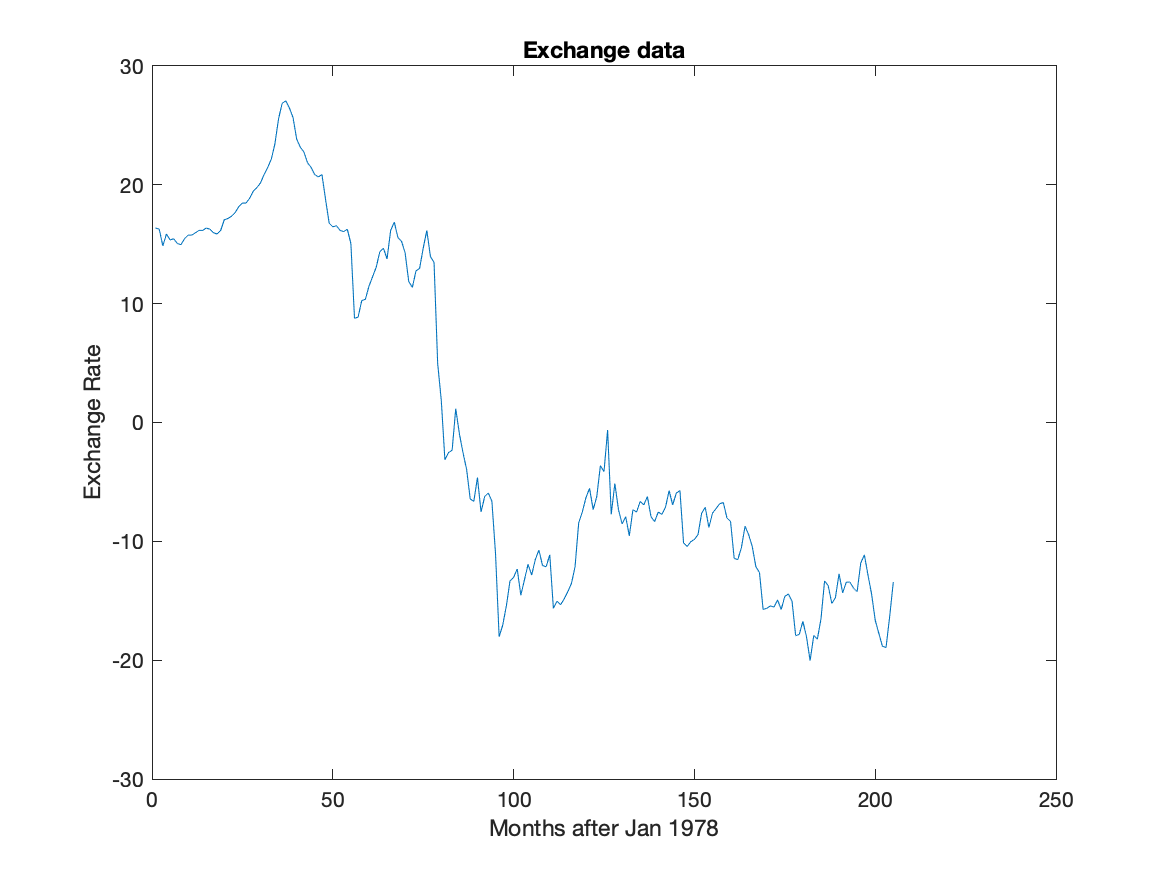
\includegraphics[width=10cm]{plots/exchangedata.png}
\centering
\caption{Monthly observations of the Australian Trade Weighted Index}
\label{fig:exchangerate}
\end{figure}

In Figure \ref{fig:exchangerate} we we can see the the monthly observations of the Australian Trade Weighted Index.
From this graph it does not appear to be a stationary process.
For an lag set to say $h = 10$, if we look at the relation between $t = 25$ and $t = 75$, we see that the covariance is positive between $X_{25}$ and $X_{35}$ and fairly strongly negatively correlated between $X_{75}$ and $X_{85}$.
This shows informally that we are probably not dealing with a stationary time series as we would expect the covariance of $\gamma_{X}(t + h, t)$ not to depend on $t$.

\begin{figure}[h!]
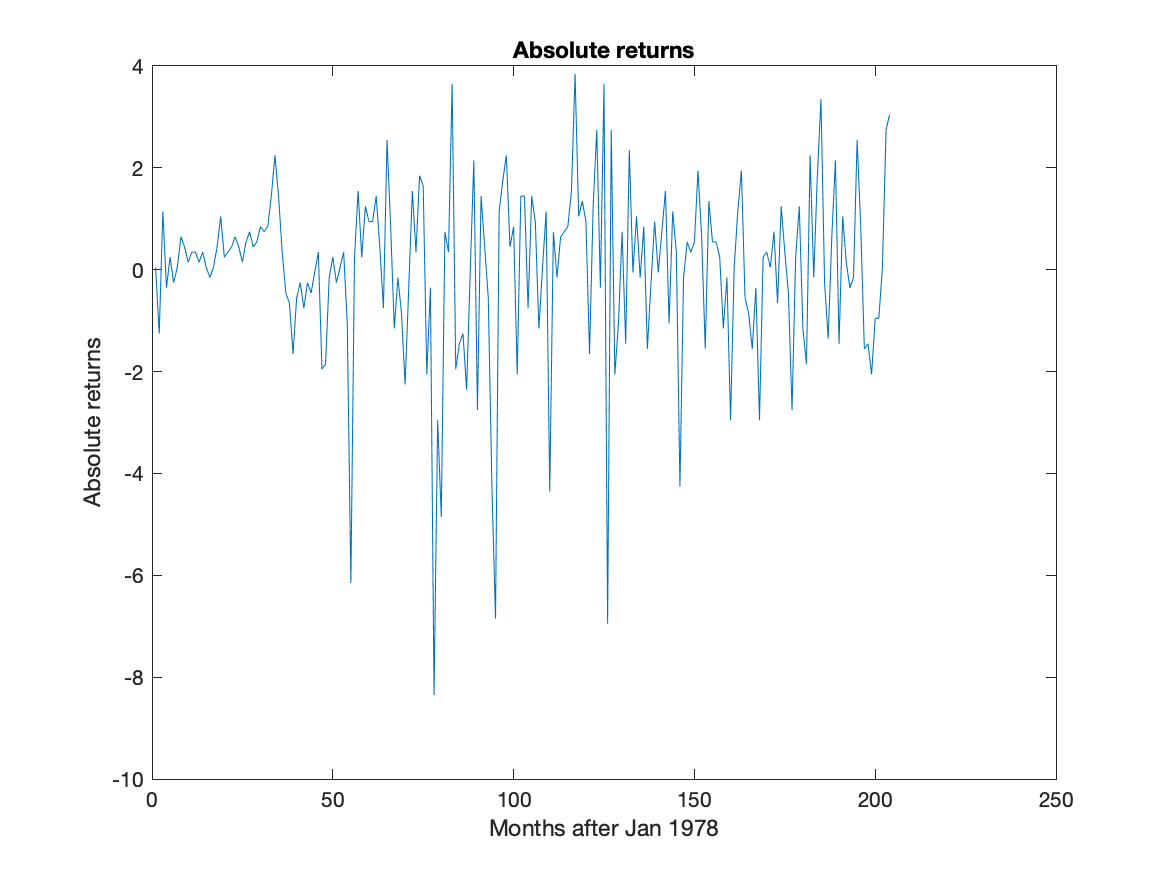
\includegraphics[width=10cm]{plots/abs_returns.png}
\centering
\caption{Absolute returns $Y_t = X_{t + 1} - X_{t}$}
\label{fig:absreturns}
\end{figure}

\begin{figure}[h!]
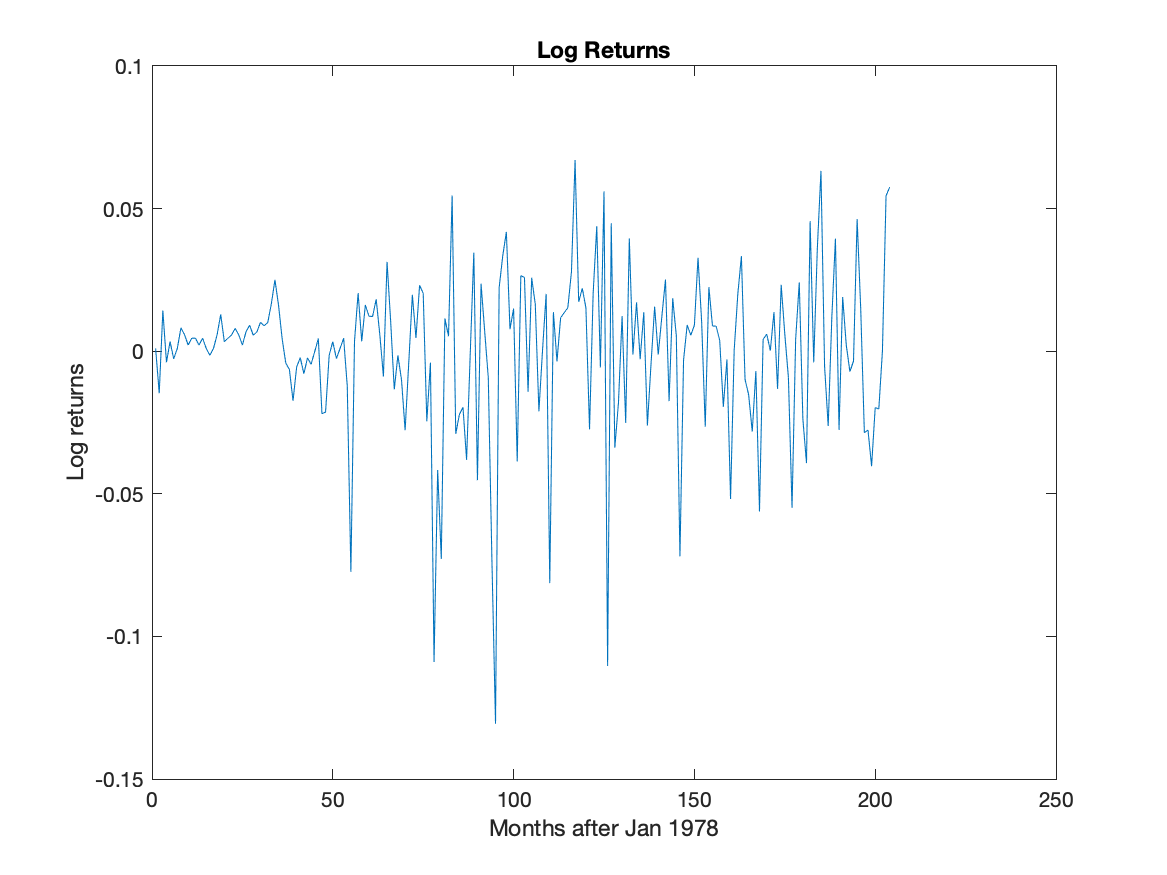
\includegraphics[width=10cm]{plots/log_returns.png}
\centering
\caption{Log returns $Z_t = \log(X_{t + 1}) - \log(X_{t})$}
\label{fig:logreturns}
\end{figure}

For both the absolute returns in Figure \ref{fig:absreturns} and the log returns in Figure \ref{fig:logreturns} it appears that the processes could be stationary.
There do not seem to be any pairs of points where the covariance of $X_{t + h}$ and $X_{t}$ would be dependent on the value of $t$.
The range of $t$ from $0 \leq t 40$ does appear slightly different from the rest of the series but not enough for us to think it would not be stationary.

\section*{Problem 5}
\subsection*{Part a}
% Show expected value the same
\begin{align*}
    E[X_t] &= E[\cos(\omega t + Y)]\\
    &= E[\cos(\omega t) \cos(Y) - sin(\omega t) sin(Y)] && \text{Sum-difference for cos}\\
    &= \cos(\omega t) E[\cos(Y)] - sin(\omega t) E[sin(Y)]\\
    &= \text{TODO: Find dist. of cos(Y) and sin(Y)}
\end{align*}



\bibliographystyle{plain}
\bibliography{references}
\end{document}
